\section{Theorie}
\label{sec:Theorie}

\subsection{Kirchhoff'sche Regel}

\subsubsection{Maschenregel}
Eine Masche beschreibt einen in sich geschlossenen Stromkreis. Die Maschenregel besagt, dass für eine Masche die Summe
aller Einzelspannungen $U_k$ an den einzelnen Bauelementen, wie zum Beispiel Ohmschen Widerständen,
gleich der angelegten Gesamtspannung $U_0$ ist.
\begin{equation}
\sum_{k}
\end{equation}

\subsubsection{Knotenregel}
Die Knotenregel besagt anschaulich, dass Ströme, die in einen Knotenpunkt
hineinfließen, auch wieder hinausfließen müssen. Im Knoten selbst dürfen also keine Ströme verschwinden,
oder neu entstehen.
\begin{equation}
\sum_{k}{I_K}=0
\end{equation}
Etwas mathematischer ausgedrückt heißt das, dass die Summe über alle eingehenden
und allen ausgehenden Strömen gleich Null sein muss.



\subsection{Wheatstonesche Brückenschaltung}
\begin{figure}
  \centering
  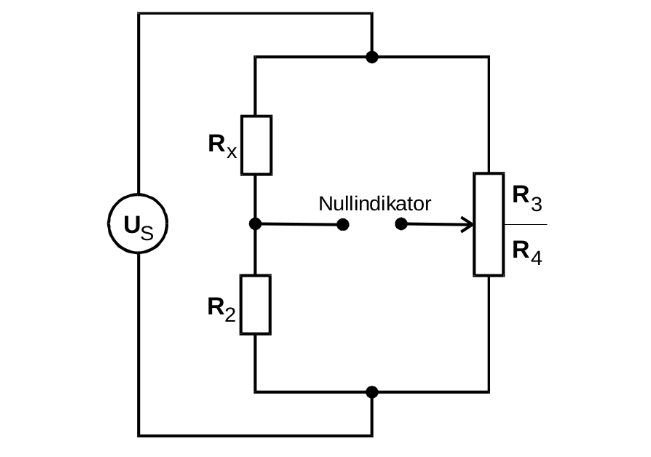
\includegraphics[width=0.9\textwidth]{Bilder/Wheatstone_bruecke.png}
  \caption{Wheatstonesche Brückenschaltung zur Bestimmung eines unbekannten Widerstands \cite{Anleitung}}
  \label{fig:wheatstonebrücke}
\end{figure}
\blindtext
\begin{equation}
  R_x=R_2 \cdot \frac{R_3}{R_4};
\label{eqn:widerstand}
\end{equation}
\subsection{Kapazitätsmessbrücke}
\begin{figure}
  \centering
  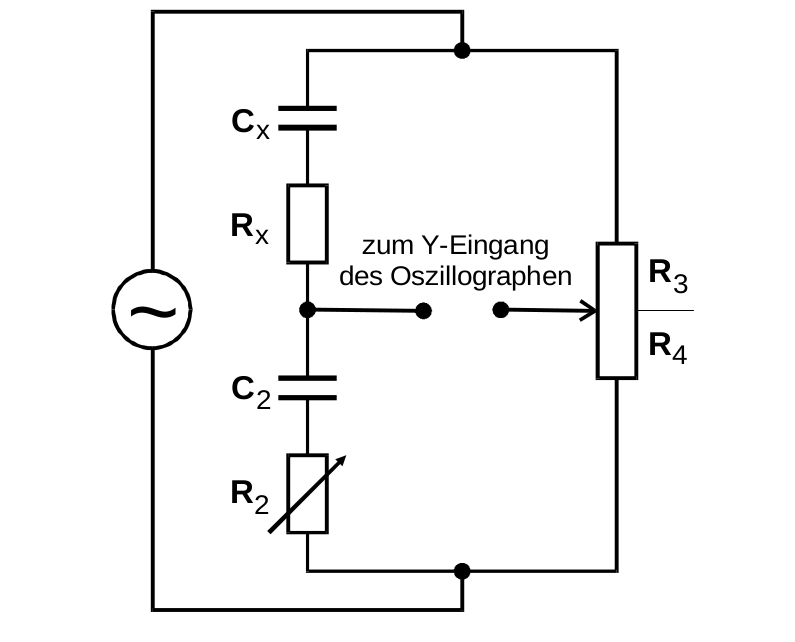
\includegraphics[width=0.9\textwidth]{Bilder/kapazitaetmessbruecke.png}
  \caption{Brückenschaltung zur Bestimmung eines unbekannten Kondensators \cite{Anleitung}}
  \label{fig:kapazitaetmessbrücke}
\end{figure}
\blindtext
\subsection{Induktivitätsmessbrücke}
\begin{figure}
  \centering
  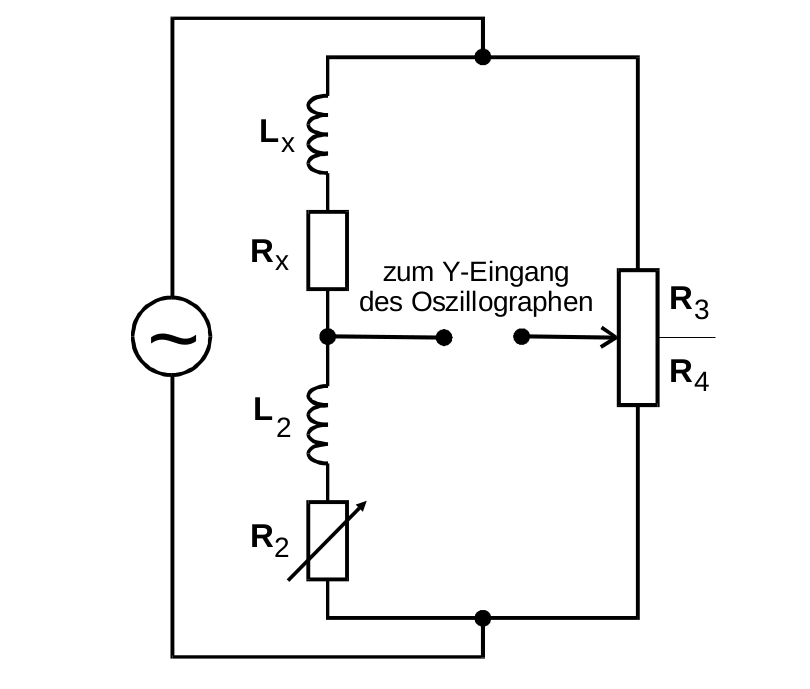
\includegraphics[width=0.9\textwidth]{Bilder/Messbruecke_Spule_mit_R.png}
  \caption{Brückenschaltung zur Bestimmung der Induktivität einer Spule  \cite{Anleitung}}
  \label{fig:induktivitätsmessbrücke}
\end{figure}
\blindtext
\subsection{Maxwell-Brücke}
\begin{figure}
  \centering
  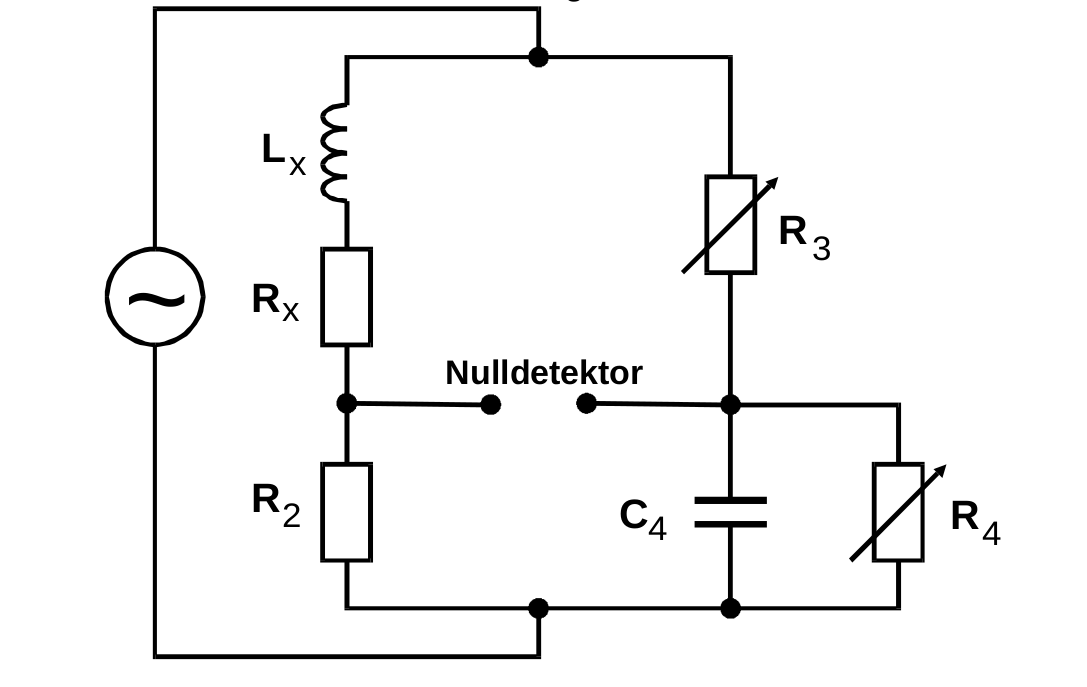
\includegraphics[width=0.9\textwidth]{Bilder/maxwell_bruecke.png}
  \caption{Maxwell-Brücke zur Bestimmung einer Induktivität \cite{Anleitung}}
  \label{fig:maxxwellbrücke}
\end{figure}

\subsection{Wien-Robinson-Brücke}
\begin{figure}
  \centering
  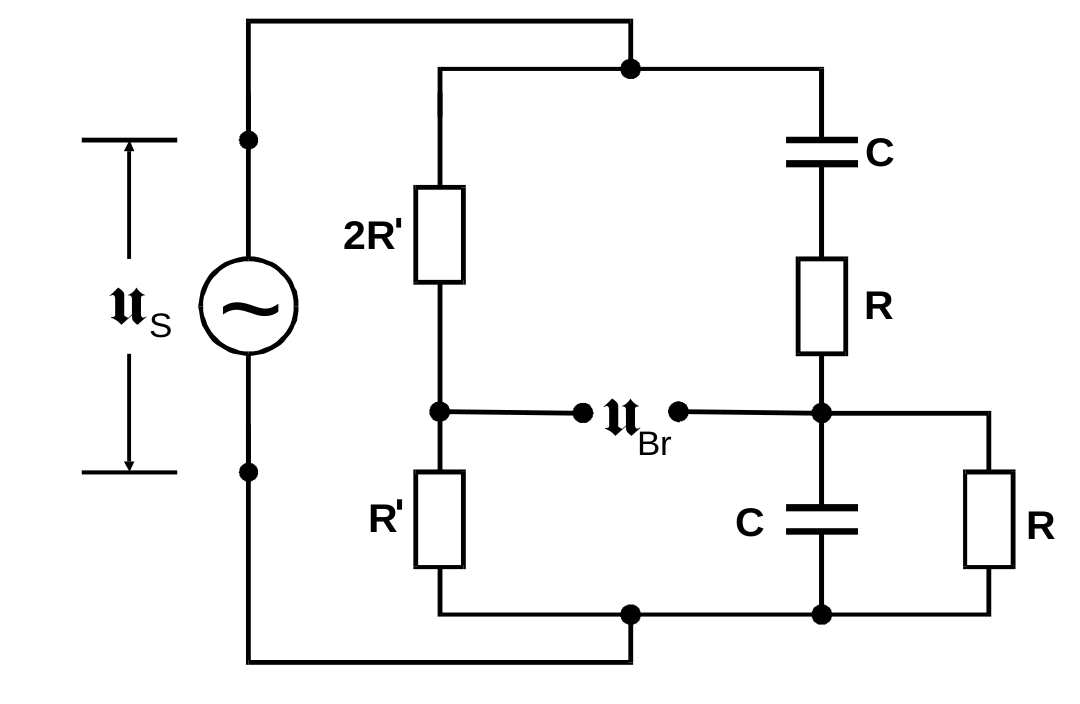
\includegraphics[width=0.9\textwidth]{Bilder/wien_robinson_bruecke.png}
  \caption{Wien-Robinson-Brücke zur Klirrfaktor-Bestimmung \cite{Anleitung}}
  \label{fig:wienrobinsonbrücke}
\end{figure}
\blindtext
\subsubsection{Klirrfaktor-Messung}
\blindtext
